\chapter{The GAN}
Developing the GAN poses many question, but the first and most important one is the fact that GANs work better
with continuos input attributes and the data present in our dataset it is not of this kind. For this we have
to apply some tricks so that our data can be given as an input of the Neural Network.
\\\\
Before diving deeper into the implementation of this process it is necessary to discuss what a GAN is.
A GAN o Generative Adversarial Network is a Neural Network used to generate synthetic data by learingn from a
given set of input data. GANs are made of two networks, a generator G and a discriminator D. The generator 
is trained to generate synthetic data from noise. The goal of the discriminator is to distinguish generated 
data from the real word data. The generator is trained iteratively until the generator is able to fool the
discriminator. GANs are really good at generating images, but they have achieved good result also in text
generation or molecule generation.
\\\\
Discriminative models aim to classify objects into predefined classes. In contrast to discriminative models, 
generative ones are used to generate data like the network traffic. Many generative models build on likelihood
maximization for a parametric probability distribution. The generator tries to mimic sample from the data 
distribution, while the discriminator has to differentiate the real and the generated samples.
Both networks are trained iteratively until the discriminator can't distinguish real and generated samples. 
The generator is never updated with real samples. The generator is fed with an input vector of noise 
\textit{z}. So it is trained using only the discriminator's gradient through backpropagation. 
Therefore it is less likely to overfit the generato by memorizing and reproduct real samples.
\begin{figure}[h]
    \centering
    \begin{subfigure}{.45\textwidth}
        \centering
        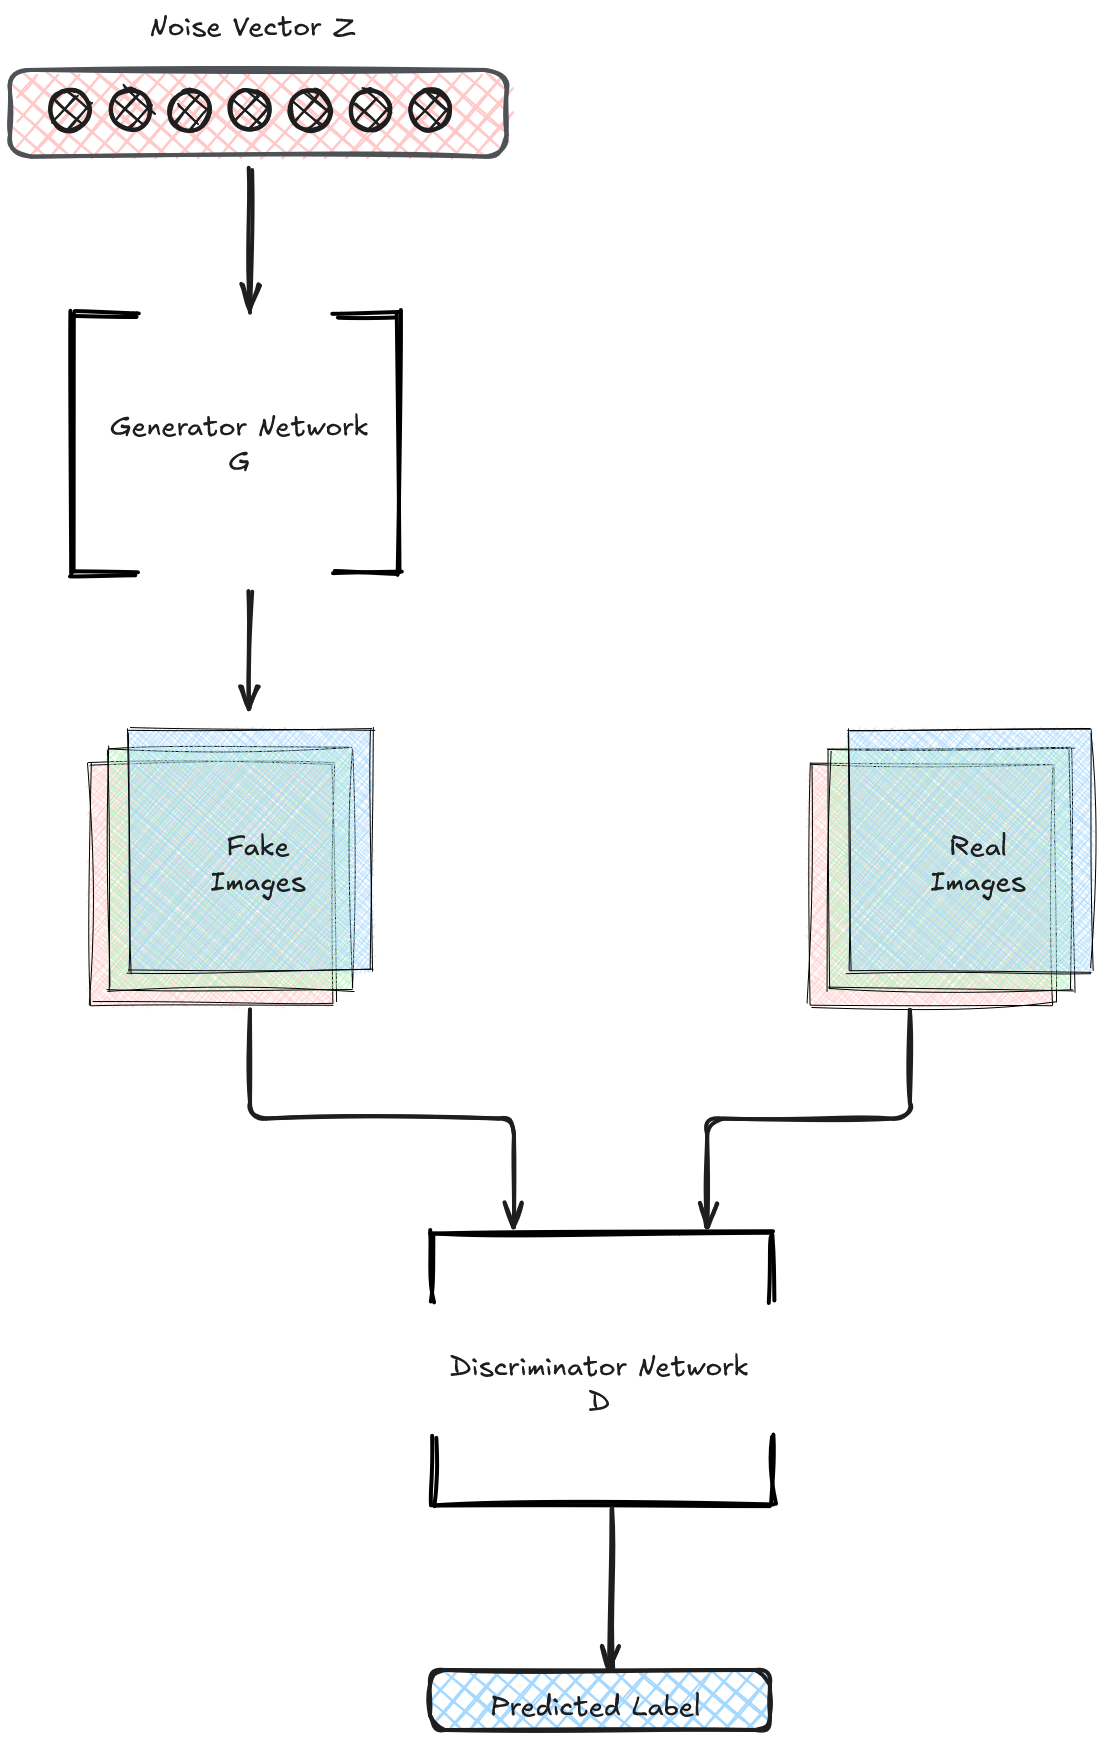
\includegraphics[width=.95\linewidth]{GAN.png}  
        %\caption{}
        \caption{Classic GAN architecture}
    \end{subfigure}
    \begin{subfigure}{.45\textwidth}
        \centering
        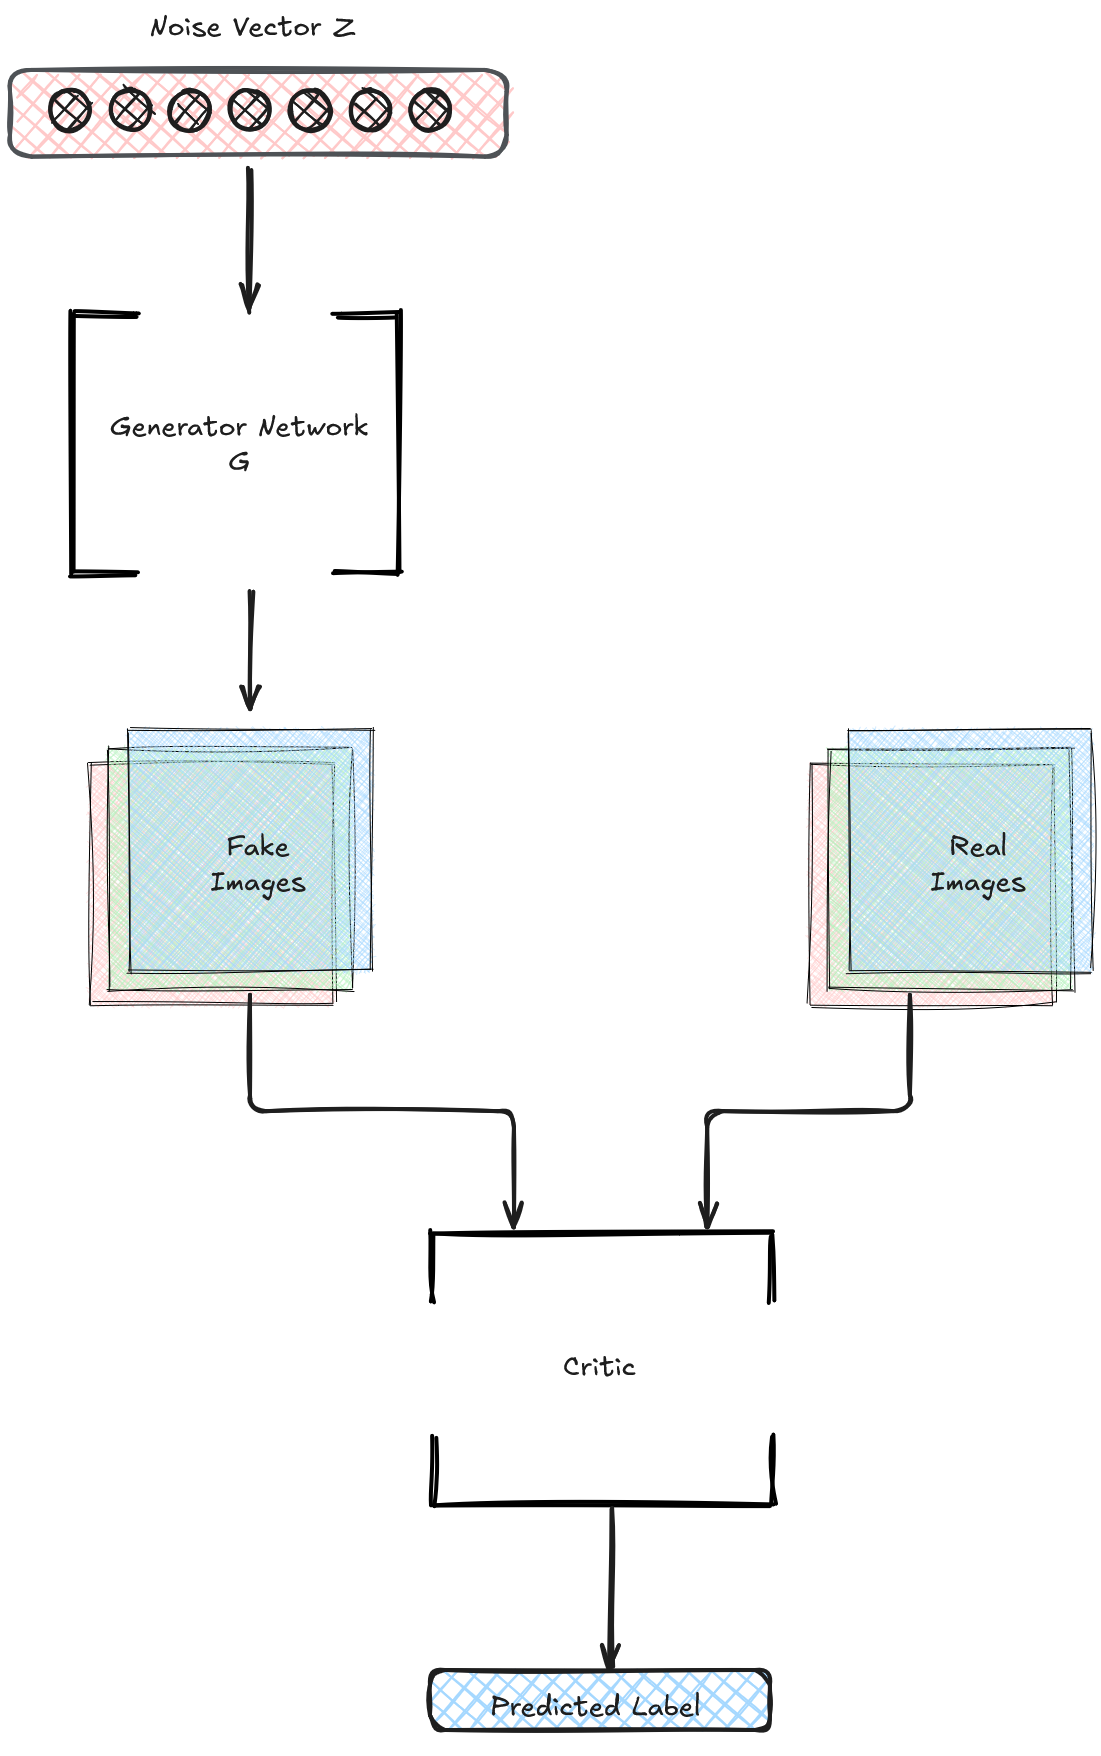
\includegraphics[width=.95\linewidth]{WGAN.png}  
        \caption{Architecture of a WGAN}
    \end{subfigure}
    \label{Architecture differences}
\end{figure}
The vanilla GANs requires the visible units to be differentiable, which is not the case for categorical 
attributes like IPs in the data used. WGANs \cite{wgan} \cite{wgan4n}, are capable of modelling discrete distributions over a continuos
latent space and have other advantages. The main difference is that WGANs uses the Earth Mover (EM) distance 
as a value function replacing the classifying discriminator network with a \textit{critic} network estimating
the distance. To solve the problem of non-convergence in the GANs, it could be useful to apply Two Time-Scale
Update (TTUR) for training GANs with arbitrary functions. For this reason we have choosen to utilize 
WGANs with TTUR.
\section{Preprocessing}
Since the packet capture network traffic that we use as input is made of by both categorical and continuous data,
we need a way to transform the categorical data into continuous ones. There are various methods to do so, one
of them is tho simply treat the attributes like IP and ports as numerical values. The second method could be
to create binary attributes from categorical ones. The last method uses IP2Vec to learna meaningful vector 
rapresentation of the categorical attributes.
\\\\
Since the first two methods are less precise, but are more simple to implement, it has been choosen to 
implement directly the third method even if it is more complex. This due to the fact of attempting to obtain
a better approximation of the input data, and this method works better than the other two.
\section{IP2Vec}
IP2Vec \cite{ip2vec} is a work inspired by Word2Vec and aims to transform IP addresses into a continuous feature space 
$\mathbb{R}^m$ such that standard similarity measure can be applied. To do that we can extract the available
context information from the network traffic. For example the \textit{IP addresses} that appear in similar
contexts will be close to each other in the feature space $\mathbb{R}^m$. This means that similar context 
imply the fact that the devices associated to thes IPs establish similar connections. 
\begin{figure}[h]
    \centering
    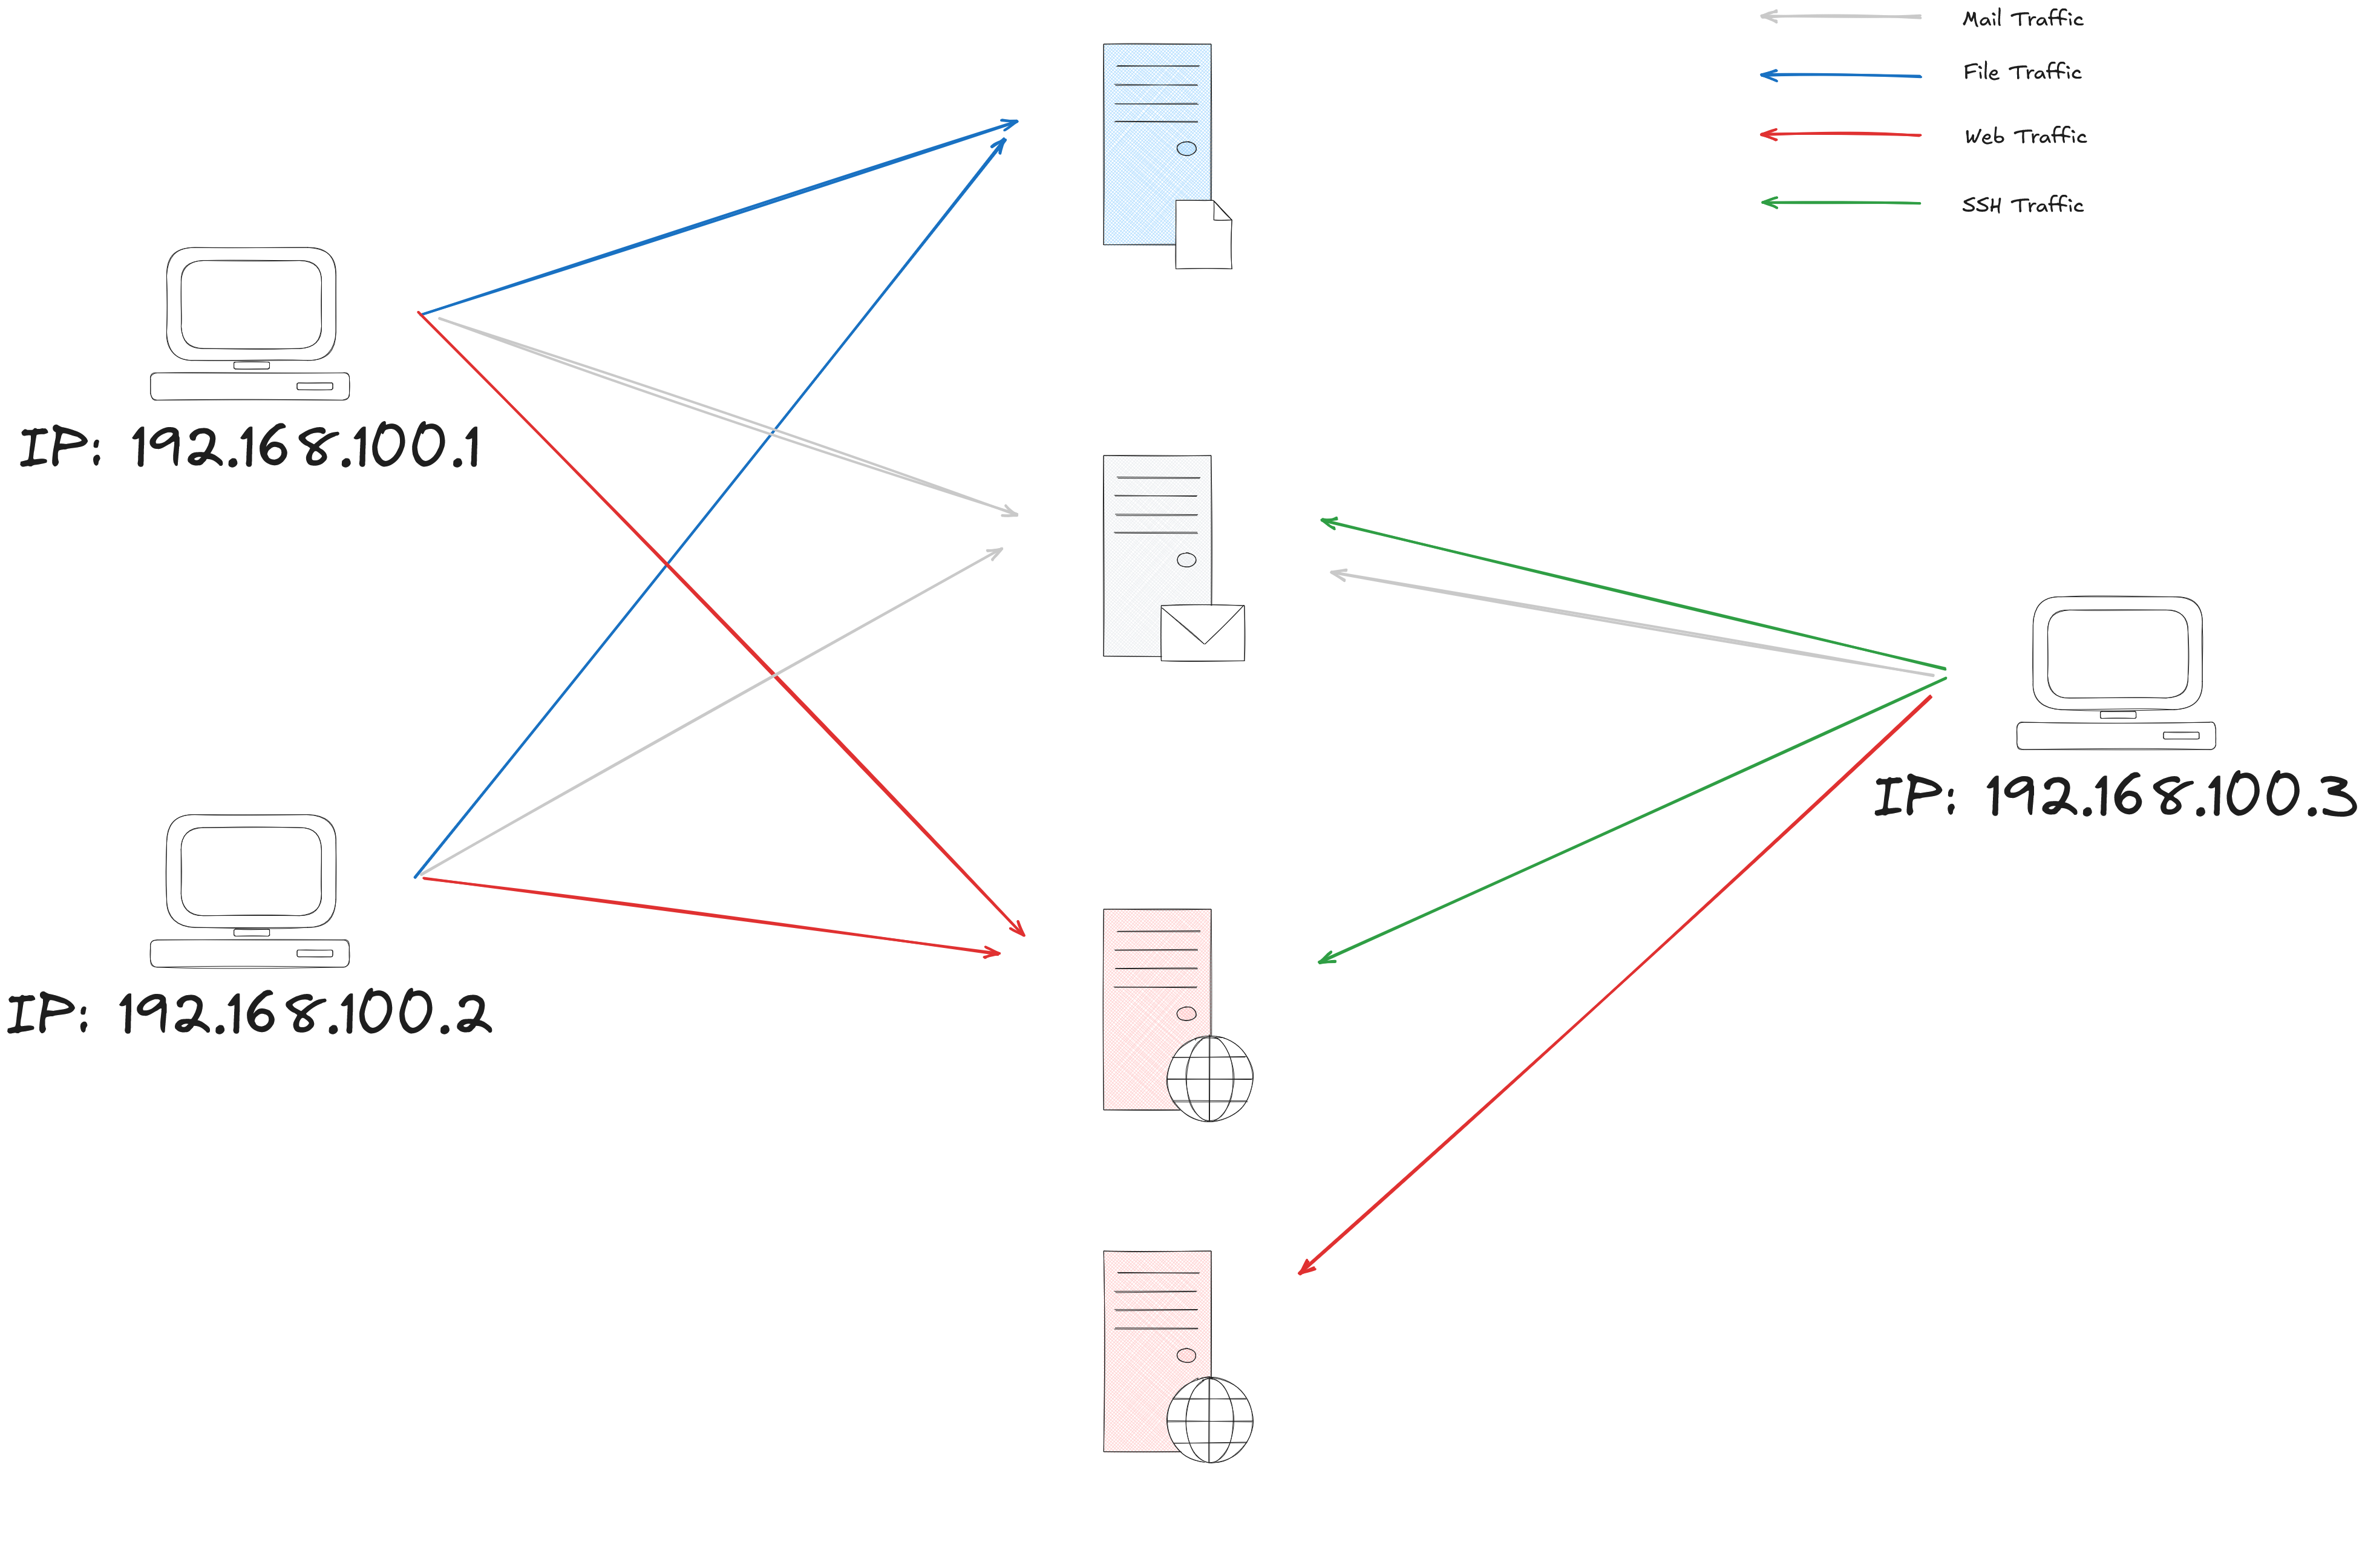
\includegraphics[width=9cm]{IP2Vec_idea.png}
    \label{IP2Vec}
    \caption{Example of connections}
\end{figure}
$\\\\$
In the figure we can see the idea of IP2Vec. The arrows denote network connections from the IPs and the 
different colors indicate different services. From the image we can tderive that the conection made 
by the devices on the left side are more similar that the ones made by, for example, the host $192.168.100.2$
and $192.168.100.3$. This due to the fact that the first couple use the sama kind of connection referred to 
the same targets and services.
\subsection{Model}
IP2Vec is based on a fully connected neural network with a single hidden layer.
\begin{figure}[h]
    \centering
    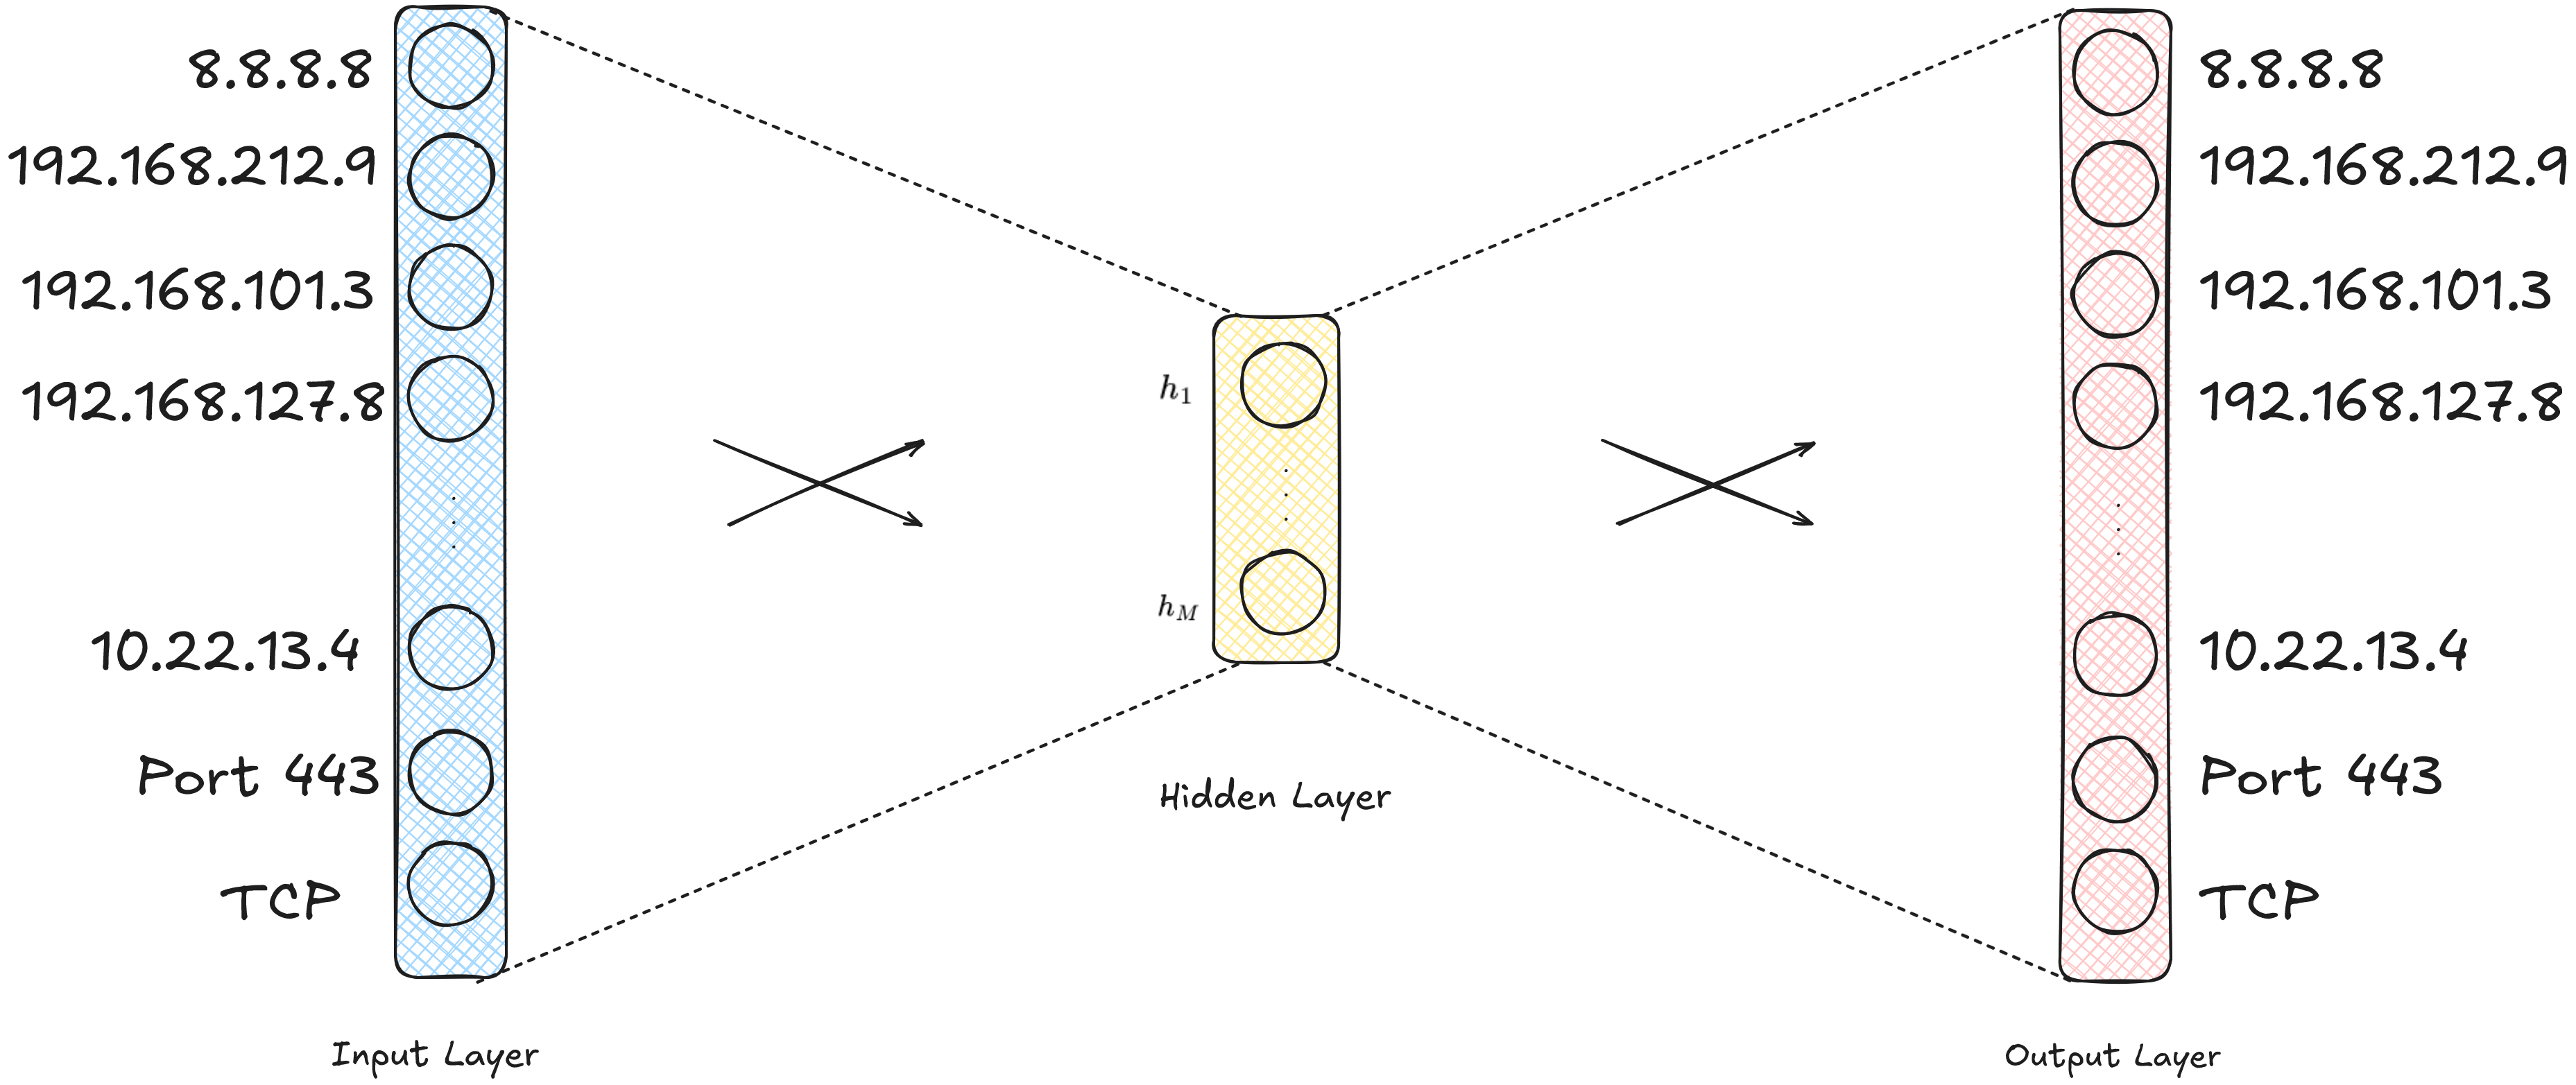
\includegraphics[width=9cm]{IP2Vec.png}
    \label{IP2Vec}
    \caption{Neural Network representation}
\end{figure}
$\\\\$
The features that are extracted from the network traffic consitute the input of the network. The features
consists of the IP addresses, destination ports and trasport protocols and contribute to create the 
vocabulary that contain all of the features that can be seen in the dataset. Since we cannot have categorical
attributes, the vocabulary is represented as a one-hot vector that has the length of the size of the 
vocabulary. 
\\\\
Each neuron in the input and output is then assigned to a specific value of the vocabulary.
The output layer uses a softmax classifier that indicates the probability of each value of the vocabulary 
that it appears in the same context as the input given. The classifier normilizes the output such that the 
sum is 1.
\subsection{Train}
In the training process the neural network is fed with the input value and it tries to predict the probability
of the other values from the vocabulary. For the trining samples the probability of the concrete output value
is 1 and 0 for all the others. The network uses back-prpagation for learning. 
\\\\
With that, we conclude the digression on how the input data is transformed in a way that can be fed to the 
GAN. Since the data generated is then reproduced as an embedding vector it needs also to be converted in a
format similar to the dataset, for that we have used a script that implement that feature

